\vspace{0.15cm}
\begin{flushleft}
	{\color{blue!50!green}\fbox{\fontfamily{qag}\bfseries\selectfont PHẦN I. Câu trắc nghiệm nhiều phương án lựa chọn (4,5 điểm)}}
	\textit{\small (Thí sinh trả lời từ câu 1 đến câu 18. Mỗi câu hỏi thí sinh chỉ chọn một phương án.)}
\end{flushleft}
\setcounter{ex}{0}
\setcounter{bt}{0}

% Câu 1
\begin{ex}
	\macau{ID: VL12-HBT2425-C01}Gọi $\Delta t$ và $\Delta T$ lần lượt là độ lớn một độ chia trên thang nhiệt độ Celsius và thang nhiệt độ Kelvin thì
	\choice
	{$\Delta t = \Delta T - 273$}
	{$\Delta t = \dfrac{1}{100} \Delta T$}
	{$\Delta t = \dfrac{1}{273} \Delta T$}
	{\True $\Delta t = \Delta T$}
	\loigiai{
		Độ lớn của một độ chia trên thang Celsius ($1^\circ\text{C}$) và trên thang Kelvin ($1\text{ K}$) là bằng nhau: $\Delta t = \Delta T$.
	}
\end{ex}

% Câu 2
\begin{ex}
	\macau{ID: VL12-HBT2425-C02}Công thức nào sau đây là công thức tổng quát của định luật I nhiệt động lực học?
	\choice
	{$A + Q = 0$}
	{$\Delta U = A$}
	{\True $\Delta U = A + Q$}
	{$\Delta U = Q$}
	\loigiai{
		Hệ thức của định luật I nhiệt động lực học: $\Delta U = A + Q$, trong đó $\Delta U$ là độ biến thiên nội năng, $A$ là công và $Q$ là nhiệt lượng mà hệ trao đổi.
	}
\end{ex}

% Câu 3
\begin{ex}
	\macau{ID: VL12-HBT2425-C03}Nhiệt lượng cần thiết cung cấp để tăng nhiệt độ của $m\text{ (kg)}$ vật liệu (có nhiệt dung riêng $c$) từ nhiệt độ $t_1$ lên tới nhiệt độ $t_2$ là
	\choice
	{\True $Q = mc(t_2 - t_1)$}
	{$Q = \lambda m$}
	{$Q = Lm$}
	{$Q = mc(t_2 + t_1)$}
	\loigiai{
		Nhiệt lượng cung cấp để vật tăng nhiệt độ từ $t_1$ đến $t_2$: $Q = mc\Delta t = mc(t_2 - t_1)$.
	}
\end{ex}

% Câu 4
\begin{ex}
	\macau{ID: VL12-HBT2425-C04}Nhiệt hóa hơi riêng là thông tin cần thiết trong việc thiết kế, chế tạo
	\choice
	{quạt điện}
	{nồi chiên không dầu}
	{\True máy điều hòa nhiệt độ}
	{nhiệt kế thủy ngân}
	\loigiai{
		Máy điều hòa nhiệt độ (và tủ lạnh) hoạt động dựa trên chu trình nhiệt sử dụng môi chất lạnh hóa hơi (thu nhiệt) và ngưng tụ (tỏa nhiệt), do đó nhiệt hóa hơi riêng của môi chất là thông số kĩ thuật cốt lõi.
	}
\end{ex}

% Câu 5
\begin{ex}
	\immini{\macau{ID: VL12-HBT2425-C05}Khi tiến hành thí nghiệm đo nhiệt hóa hơi riêng của nước, bạn Việt sử dụng các dụng cụ thí nghiệm như hình vẽ và thực hiện các thao tác sau:
	\begin{enumerate}[(1)]
		\item Đun sôi nước trong bình nhiệt lượng kế. Sau mỗi khoảng thời gian 2 phút, đọc số đo công suất trên oát kế, khối lượng nước trong bình trên cân. Ghi kết quả vào bảng.
		\item Bật nguồn điện.
		\item Nối oát kế với điện trở và nguồn điện.
		\item Tháo nắp bình ra khỏi nhiệt lượng kế.
		\item Đặt dây điện trở vào nhiệt lượng kế sao cho toàn bộ dây chìm trong nước.
		\item Đặt nhiệt lượng kế lên cân. Đổ nước nóng vào nhiệt lượng kế. Xác định khối lượng nước trong bình.
		\item Tắt nguồn điện.
	\end{enumerate}
	Trình tự thao tác thí nghiệm đúng là
	\choice
	{(7), (6), (5), (4), (3), (2), (1)}
	{(2), (3), (4), (5), (6), (7), (1)}
	{(1), (2), (3), (4), (5), (6), (7)}
	{\True (6), (4), (3), (5), (2), (1), (7)}}{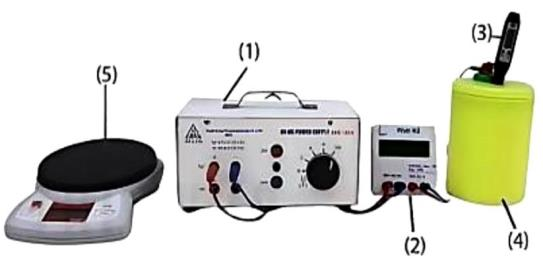
\includegraphics[width=4.0cm]{figures/fig_cau05.png}}
	\loigiai{
		Trình tự đo chuẩn: Cân xác định khối lượng nước ban đầu (6) $\to$ Tháo nắp (4) $\to$ Nối mạch điện (3) $\to$ Đặt dây điện trở chìm trong nước (5) $\to$ Bật nguồn (2) $\to$ Đun sôi và ghi số liệu theo chu kì (1) $\to$ Tắt nguồn kết thúc thí nghiệm (7).
	}
\end{ex}

% Câu 6
\begin{ex}
	\macau{ID: VL12-HBT2425-C06}Chọn cụm từ thích hợp nhất điền vào chỗ trống: ``\dots của một chất là nhiệt lượng cần để làm cho một kilôgam chất đó nóng chảy hoàn toàn ở nhiệt độ nóng chảy''.
	\choice
	{Nhiệt hoá hơi riêng}
	{Nhiệt hoá hơi}
	{\True Nhiệt nóng chảy riêng}
	{Nhiệt dung riêng}
	\loigiai{
		Theo định nghĩa: Nhiệt nóng chảy riêng của một chất là nhiệt lượng cần để làm cho một kilôgam chất đó nóng chảy hoàn toàn ở nhiệt độ nóng chảy: $\lambda = \dfrac{Q}{m}$.
	}
\end{ex}

% Câu 7
\begin{ex}
	\macau{ID: VL12-HBT2425-C07}Điều nào sau đây đúng khi nói về cấu trúc của thể rắn?
	\choice
	{Các phân tử chỉ dao động quanh vị trí cân bằng và vị trí cân bằng này chuyển động}
	{Sự sắp xếp của các phân tử không có trật tự}
	{\True Các phân tử chỉ dao động quanh vị trí cân bằng cố định}
	{Khoảng cách giữa các phân tử rất xa nhau (cỡ hàng chục lần kích thước phân tử)}
	\loigiai{
		Trong chất rắn, lực tương tác phân tử rất mạnh, các phân tử liên kết chặt chẽ và chỉ dao động nhiệt quanh các vị trí cân bằng cố định trong không gian.
	}
\end{ex}

% Câu 8
\begin{ex}
	\macau{ID: VL12-HBT2425-C08}Câu nào sau đây nói về nhiệt lượng là \textbf{không đúng}?
	\choice
	{Đơn vị nhiệt lượng cũng là đơn vị nội năng}
	{\True Một vật lúc nào cũng có nội năng, do đó lúc nào cũng có nhiệt lượng}
	{Nhiệt lượng là số đo độ biến thiên nội năng của vật trong quá trình truyền nhiệt}
	{Nhiệt lượng không phải là nội năng}
	\loigiai{
		Nhiệt lượng không phải là một dạng năng lượng tồn tại độc lập trong vật mà chỉ là số đo phần năng lượng nhiệt được trao đổi trong quá trình truyền nhiệt. Vật không chứa ``nhiệt lượng'', mà chỉ chứa ``nội năng''.
	}
\end{ex}

% Câu 9
\begin{ex}
	\immini{\macau{ID: VL12-HBT2425-C09}Nhiệt kế ở hình bên đang chỉ số đo bằng bao nhiêu theo thang nhiệt độ Kelvin?
	\choice
	{$60\text{ K}$}
	{$280\text{ K}$}
	{$15\text{ K}$}
	{\True $288\text{ K}$}}{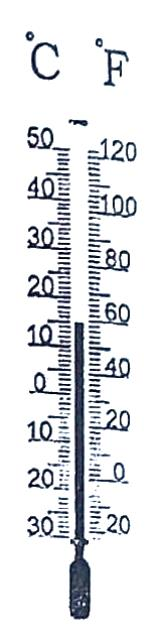
\includegraphics[width=1.6cm]{figures/fig_cau09.png}}
	\loigiai{
		Quan sát vạch chia của nhiệt kế Celsius trong hình, mức chất lỏng dừng lại ở vạch $15^\circ\text{C}$.\\
		Chuyển đổi sang thang Kelvin:
		\[
		T = t + 273{,}15 \approx 15 + 273 = 288\text{ K}.
		\]
	}
\end{ex}

% Câu 10
\begin{ex}
	\macau{ID: VL12-HBT2425-C10}Chuyển động nào dưới đây \textbf{không cần} đến sự biến đổi nhiệt lượng thành công?
	\choice
	{Sự bật lên của nắp ấm khi nước sôi}
	{\True Chiếc thuyền trôi theo dòng sông}
	{Chuyển động quay của đèn kéo quân}
	{Sự bay lên của khí cầu nhờ đốt nóng khí}
	\loigiai{
		Chiếc thuyền trôi theo dòng sông là nhờ động năng của dòng chảy tự nhiên (cơ năng), hoàn toàn không có sự biến đổi nhiệt lượng thành công cơ học.
	}
\end{ex}

% Câu 11
\begin{ex}
	\immini{\macau{ID: VL12-HBT2425-C11}Một học sinh thực hiện thí nghiệm đo nhiệt dung riêng của nước với sơ đồ bố trí thí nghiệm như hình vẽ. Trong đó, bình nhiệt lượng kế chứa $150\text{ g}$ nước có nhiệt độ ban đầu là $62^\circ\text{C}$. Số chỉ vôn kế và ampe kế lần lượt là $1{,}6\text{ V}$ và $2{,}5\text{ A}$. Sau khoảng thời gian $8\text{ phút } 50\text{ giây}$ thì thấy nhiệt độ của nước tăng lên $65{,}5^\circ\text{C}$. Bỏ qua nhiệt lượng mà bình nhiệt lượng kế và đũa khuấy thu vào. Nhiệt dung riêng của nước trong thí nghiệm này xấp xỉ bằng
	\choice
	{$4083\text{ J/(kg}\cdot\text{K)}$}
	{\True $4038\text{ J/(kg}\cdot\text{K)}$}
	{$4032\text{ J/(kg}\cdot\text{K)}$}
	{$4023\text{ J/(kg}\cdot\text{K)}$}}{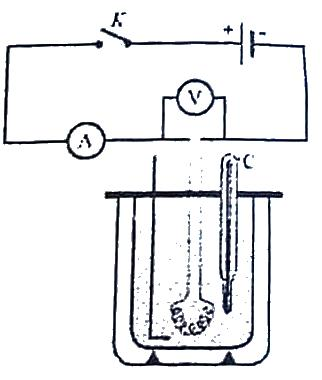
\includegraphics[width=3.2cm]{figures/fig_cau11.png}}
	\loigiai{
		Thời gian đun: $\tau = 8 \times 60 + 50 = 530\text{ s}$.\\
		Nhiệt lượng tỏa ra từ dây nung:
		\[
		Q = U I \tau = 1{,}6 \times 2{,}5 \times 530 = 2120\text{ J}.
		\]
		Nhiệt lượng nước thu vào:
		\[
		Q = mc\Delta t \Rightarrow 2120 = 0{,}15 \times c \times (65{,}5 - 62) = 0{,}525 c.
		\]
		Suy ra:
		\[
		c = \dfrac{2120}{0{,}525} \approx 4038{,}1\text{ J/(kg}\cdot\text{K)}.
		\]
	}
\end{ex}

% Câu 12
\begin{ex}
	\macau{ID: VL12-HBT2425-C12}Cho hai vật có nhiệt độ khác nhau tiếp xúc với nhau. Nhiệt được tự truyền từ
	\choice
	{vật có khối lượng lớn hơn sang vật có khối lượng nhỏ hơn}
	{vật ở trên cao sang vật ở dưới thấp}
	{vật có nhiệt độ thấp hơn sang vật có nhiệt độ cao hơn}
	{\True vật có nhiệt độ cao hơn sang vật có nhiệt độ thấp hơn}
	\loigiai{
		Theo nguyên lí truyền nhiệt tự nhiên, nhiệt chỉ có thể tự truyền từ vật có nhiệt độ cao hơn sang vật có nhiệt độ thấp hơn cho đến khi đạt trạng thái cân bằng nhiệt.
	}
\end{ex}

% Câu 13
\begin{ex}
	\macau{ID: VL12-HBT2425-C13}Nhiệt dung riêng của một chất là nhiệt lượng cần thiết cung cấp để
	\choice
	{\True $1\text{ kg}$ chất đó tăng thêm $1\text{ K}$ (hoặc $1^\circ\text{C}$)}
	{$1\text{ m}^3$ chất đó tăng thêm $1\text{ K}$ (hoặc $1^\circ\text{C}$)}
	{$1\text{ mol}$ chất đó tăng thêm $1\text{ K}$ (hoặc $1^\circ\text{C}$)}
	{$1$ phân tử chất đó tăng thêm $1\text{ K}$ (hoặc $1^\circ\text{C}$)}
	\loigiai{
		Nhiệt dung riêng $c$ của một chất là nhiệt lượng cần truyền cho $1\text{ kg}$ chất đó để nhiệt độ của nó tăng thêm $1\text{ K}$ (hoặc $1^\circ\text{C}$).
	}
\end{ex}

% Câu 14
\begin{ex}
	\immini{\macau{ID: VL12-HBT2425-C14}Sự biến thiên nhiệt độ theo thời gian của khối nước đá khi được cung cấp nhiệt lượng được biểu diễn theo đồ thị hình bên. Thời gian nóng chảy của nước đá xảy ra trong
	\choice
	{$1\text{ phút}$}
	{\True $3\text{ phút}$}
	{$7\text{ phút}$}
	{$4\text{ phút}$}}{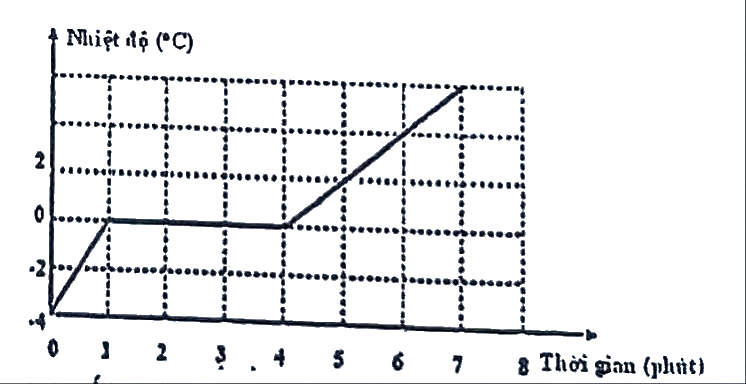
\includegraphics[width=4.0cm]{figures/fig_cau13.png}}
	\loigiai{
		Trên đồ thị, quá trình nóng chảy của nước đá diễn ra ở nhiệt độ không đổi $0^\circ\text{C}$, tương ứng với đoạn nằm ngang từ thời điểm $t = 1\text{ phút}$ đến $t = 4\text{ phút}$.\\
		Khoảng thời gian nóng chảy: $\Delta t = 4 - 1 = 3\text{ phút}$.
	}
\end{ex}

% Câu 15
\begin{ex}
	\macau{ID: VL12-HBT2425-C15}Bạn Khoa muốn đun sôi $1{,}5\text{ lít}$ nước bằng bếp từ. Do sơ suất nên bạn quên không tắt bếp khi nước sôi. Biết nhiệt hóa hơi riêng của nước là $2{,}3 \times 10^6\text{ J/kg}$ và khối lượng riêng của nước là $10^3\text{ kg/m}^3$. Nhiệt lượng đã làm hóa hơi $1\text{ lít}$ nước trong ấm do sơ suất đó là
	\choice
	{$1{,}53 \times 10^6\text{ J}$}
	{$1{,}5 \times 10^6\text{ J}$}
	{\True $2{,}3 \times 10^6\text{ J}$}
	{$3{,}45 \times 10^6\text{ J}$}
	\loigiai{
		Khối lượng của $1\text{ lít}$ nước bị hóa hơi:
		\[
		m = V \times D = 1 \times 10^{-3} \times 10^3 = 1\text{ kg}.
		\]
		Nhiệt lượng làm hóa hơi lượng nước này:
		\[
		Q = Lm = 2{,}3 \times 10^6 \times 1 = 2{,}3 \times 10^6\text{ J}.
		\]
	}
\end{ex}

% Câu 16
\begin{ex}
	\macau{ID: VL12-HBT2425-C16}Hiện tượng nào sau đây \textbf{không} liên quan đến sự nóng chảy?
	\choice
	{Thép được nấu trong lò luyện kim}
	{Viên nước đá đang tan dần trong cốc nước chanh}
	{\True Ngọn đèn dầu đang cháy}
	{Mỡ lợn tan ra khi bị đun nóng}
	\loigiai{
		Ngọn đèn dầu cháy là phản ứng oxi hóa hóa học của hơi dầu với oxi trong không khí, không liên quan đến sự chuyển từ thể rắn sang thể lỏng (sự nóng chảy).
	}
\end{ex}

% Câu 17
\begin{ex}
	\macau{ID: VL12-HBT2425-C17}Khi nói về sự đông đặc của các chất, kết luận nào dưới đây \textbf{không đúng}?
	\choice
	{\True Nhiệt độ nóng chảy của một chất luôn cao hơn nhiệt độ đông đặc của chất ấy}
	{Trong suốt thời gian đông đặc nhiệt độ của vật không thay đổi}
	{Phần lớn các chất nóng chảy ở một nhiệt độ xác định}
	{Nhiệt độ đông đặc của các chất khác nhau thì khác nhau}
	\loigiai{
		Đối với mỗi chất rắn kết tinh tinh khiết, nhiệt độ nóng chảy bằng chính nhiệt độ đông đặc ở cùng áp suất xác định. Khẳng định ``nhiệt độ nóng chảy luôn cao hơn nhiệt độ đông đặc'' là không đúng.
	}
\end{ex}

% Câu 18
\begin{ex}
	\macau{ID: VL12-HBT2425-C18}Trong suốt thời gian nước sôi, nhiệt độ của nước
	\choice
	{giảm dần}
	{ban đầu tăng rồi sau đó giảm}
	{\True không thay đổi}
	{tăng dần}
	\loigiai{
		Trong suốt quá trình sôi ở áp suất tiêu chuẩn, toàn bộ nhiệt lượng cung cấp được dùng để phá vỡ các liên kết phân tử chuyển nước sang thể hơi, do đó nhiệt độ của nước duy trì không đổi ở $100^\circ\text{C}$.
	}
\end{ex}

\vspace{0.15cm}
\begin{flushleft}
	{\color{blue!50!green}\fbox{\fontfamily{qag}\bfseries\selectfont PHẦN II. Câu trắc nghiệm đúng sai (4,0 điểm)}}
	\textit{\small (Thí sinh trả lời từ câu 1 đến câu 4. Trong mỗi ý a), b), c), d) ở mỗi câu, thí sinh chọn đúng hoặc sai.)}
\end{flushleft}
\setcounter{ex}{0}

% Câu 19
\begin{ex}
	\immini{\macau{ID: VL12-HBT2425-C19}Sự biến thiên nhiệt độ của khối nước đá đựng trong ấm điện theo nhiệt lượng cung cấp được cho trên đồ thị hình bên.
	\choiceTF
	{Khi nhiệt lượng cung cấp cho khối nước đá đạt $180\text{ kJ}$ thì nước bắt đầu sôi}
	{Ban đầu cần cung cấp nhiệt lượng $100\text{ J}$ để nước đá nóng chảy hoàn toàn}
	{\True Trong quá trình cung cấp nhiệt lượng cho khối đá từ $0$ đến $100\text{ kJ}$, nhiệt độ nước vẫn là $0^\circ\text{C}$ không thay đổi}
	{Để đun nước từ $0^\circ\text{C}$ lên đến $100^\circ\text{C}$ cần cung cấp nhiệt lượng $300\text{ kJ}$}}{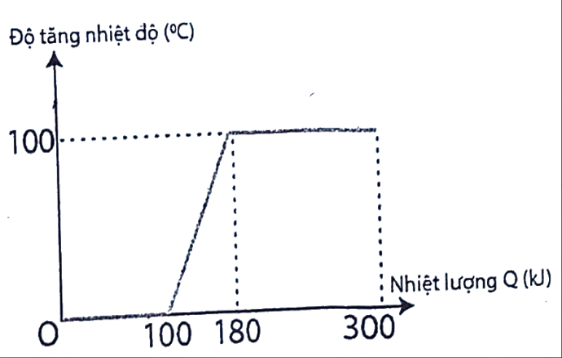
\includegraphics[width=4.0cm]{figures/fig_cau19.png}}
	\loigiai{
	\begin{itemchoice}
		\itemch Từ đồ thị, đoạn đun nước từ $0^\circ\text{C}$ lên $100^\circ\text{C}$ bắt đầu từ mốc $Q = 100\text{ kJ}$ và kết thúc ở $Q = 280\text{ kJ}$. Do đó nước chỉ bắt đầu sôi khi nhiệt lượng tích lũy đạt $280\text{ kJ}$ chứ không phải $180\text{ kJ}$.
		\itemch Nhiệt lượng cần để làm nóng chảy hoàn toàn nước đá là $Q_{nc} = 100\text{ kJ} = 100\,000\text{ J}$, không phải $100\text{ J}$.
		\itemch Đoạn nằm ngang từ $0$ đến $100\text{ kJ}$ ứng với quá trình chuyển thể ở $0^\circ\text{C}$, trong suốt giai đoạn này nhiệt độ duy trì không đổi ở $0^\circ\text{C}$.		\itemch Nhiệt lượng cần cung cấp để đun nước từ $0^\circ\text{C}$ lên $100^\circ\text{C}$ là $\Delta Q = 280 - 100 = 180\text{ kJ}$, không phải $300\text{ kJ}$.
	\end{itemchoice}
	}
\end{ex}

% Câu 20
\begin{ex}
	\macau{ID: VL12-HBT2425-C20}Trong các phát biểu sau đây về chất ở thể rắn:
	\choiceTF
	{\True Ở thể rắn, các phân tử rất gần nhau (khoảng cách giữa các phân tử cỡ kích thước phân tử)}
	{\True Lực tương tác giữa các phân tử thể rắn rất mạnh giữ cho chúng không di chuyển tự do mà chỉ có thể dao động xung quanh vị trí cân bằng xác định}
	{Vật rắn có thể tích và hình dạng riêng không xác định}
	{Các phân tử ở thể rắn sắp xếp hoàn toàn không có trật tự}
	\loigiai{
	\begin{itemchoice}
		\itemch Ở thể rắn mật độ phân tử rất lớn, khoảng cách giữa các phân tử xấp xỉ cỡ kích thước phân tử ($10^{-10}\text{ m}$).		\itemch Lực tương tác liên kết rất lớn, cố định các phân tử dao động quanh các nút mạng/vị trí cân bằng xác định.
		\itemch Vật rắn có thể tích và hình dạng riêng hoàn toàn xác định.
		\itemch Chất rắn kết tinh có cấu trúc mạng tinh thể với trật tự tuần hoàn xa rất chặt chẽ.
	\end{itemchoice}
	}
\end{ex}

% Câu 21
\begin{ex}
	\macau{ID: VL12-HBT2425-C21}Một người nặng $54\text{ kg}$ ăn một chiếc bánh có năng lượng $54\text{ kcal}$ cho bữa sáng. Giả sử $1\text{ cal} = 4{,}2\text{ J}$, lấy $g = 10\text{ m/s}^2$.
	\choiceTF
	{\True Năng lượng của chiếc bánh tương đương với $226{,}8\text{ kJ}$}
	{\True Nếu cơ thể con người có hiệu suất chuyển đổi thế năng hoá học thành cơ năng là $25\%$ thì để tiêu hao hết lượng năng lượng của chiếc bánh đó người này phải leo $700$ bậc thang (biết độ cao mỗi bậc thang là $15\text{ cm}$)}
	{\True Theo nghiên cứu, trung bình một người trưởng thành nặng khoảng $50 - 60\text{ kg}$, khi chạy bộ sẽ đốt cháy $12\text{ kcal/phút}$ nếu duy trì tốc độ $5\text{ km/h}$. Nếu đốt cháy hết năng lượng của chiếc bánh cung cấp bằng việc chạy bộ thì người này phải chạy với tốc độ đó trong $4{,}5\text{ phút}$}
	{Để tiêu hao hết lượng năng lượng của chiếc bánh đó (với hiệu suất $100\%$) người này phải leo $2768$ bậc thang trên một cầu thang rất cao, biết độ cao mỗi bậc thang là $15\text{ cm}$}
	\loigiai{
	\begin{itemchoice}
		\itemch Năng lượng chiếc bánh: $E = 54 \times 10^3 \times 4{,}2 = 226\,800\text{ J} = 226{,}8\text{ kJ}$.
		\itemch Cơ năng sinh ra: $A = 0{,}25 \times 226\,800 = 56\,700\text{ J}$.\\
		Mặt khác công leo $N$ bậc thang: $A = mgh = 54 \times 10 \times (N \times 0{,}15) = 81N$.\\
		Suy ra số bậc thang: $N = \dfrac{56\,700}{81} = 700$ bậc.
		\itemch Thời gian chạy bộ cần thiết: $t = \dfrac{54\text{ kcal}}{12\text{ kcal/phút}} = 4{,}5\text{ phút}$.
		\itemch Với hiệu suất $100\%$, số bậc thang cần leo là $N = \dfrac{226\,800}{81} = 2800$ bậc, không phải $2768$ bậc.
	\end{itemchoice}
	}
\end{ex}

% Câu 22
\begin{ex}
	\immini{\macau{ID: VL12-HBT2425-C22}Một xi lanh nằm ngang được chia thành hai phần bởi pit-tông cách nhiệt như hình vẽ. Người ta truyền nhiệt lượng $50\text{ J}$ cho khí bên ngăn $A$ thì pit-tông chuyển động đều một đoạn $20\text{ cm}$ về phía ngăn $B$. Biết lực ma sát giữa xi lanh và pit-tông là $16\text{ N}$.
	\choiceTF
	{Tổng độ biến thiên nội năng của khí ở cả ngăn $A$ và ngăn $B$ là $50\text{ J}$}
	{Khí ở ngăn $A$ nhận được một công là $3{,}2\text{ J}$}
	{\True Khí ở ngăn $B$ nhận một công bằng độ biến thiên nội năng của nó}
	{Độ biến thiên nội năng của khí ở ngăn $A$ lớn hơn $50\text{ J}$}}{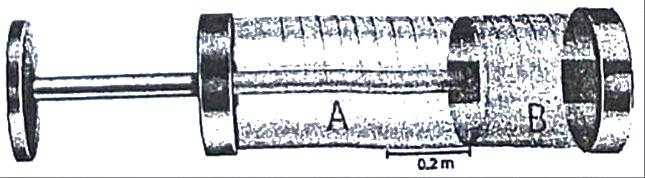
\includegraphics[width=4.0cm]{figures/fig_cau22.png}}
	\loigiai{
	\begin{itemchoice}
		\itemch Công ma sát tiêu hao cơ năng biến thành nhiệt tỏa ra môi trường: $A_{ms} = F_{ms} \times s = 16 \times 0{,}2 = 3{,}2\text{ J}$. Do đó tổng biến thiên nội năng của khí trong hai ngăn là $\Delta U_A + \Delta U_B = Q - A_{ms} = 50 - 3{,}2 = 46{,}8\text{ J}$.
		\itemch Khí ngăn $A$ dãn nở đẩy pit-tông nên khí ngăn $A$ thực hiện công ($A_A < 0$).
		\itemch Ngăn $B$ cách nhiệt ($Q_B = 0$) và bị nén nên theo định luật I: $\Delta U_B = A_B$ (độ biến thiên nội năng bằng công nhận được).
		\itemch Khí ngăn $A$ nhận nhiệt $Q_A = 50\text{ J}$ và dãn nở sinh công $A'_A > 0$ nên $\Delta U_A = Q_A - A'_A < 50\text{ J}$.
	\end{itemchoice}
	}
\end{ex}

\vspace{0.15cm}
\begin{flushleft}
	{\color{blue!50!green}\fbox{\fontfamily{qag}\bfseries\selectfont PHẦN III. Câu trắc nghiệm trả lời ngắn (1,5 điểm)}}
	\textit{\small (Thí sinh trả lời từ câu 1 đến câu 6.)}
\end{flushleft}
\setcounter{ex}{0}

% Câu 23
\begin{ex}
	\macau{ID: VL12-HBT2425-C23}Một viên đạn đại bác có khối lượng $5\text{ kg}$ khi rơi tới đích có vận tốc $17\text{ m/s}$. Nếu toàn bộ động năng của nó biến thành nội năng thì nhiệt lượng tỏa ra lúc va chạm bằng bao nhiêu Jun (làm tròn kết quả đến chữ số hàng phần mười)?

	\par\shortans[oly]{722{,}5}
	\loigiai{
		Toàn bộ động năng chuyển hóa thành nhiệt lượng tỏa ra:
		\[
		Q = W_đ = \dfrac{1}{2} m v^2 = \dfrac{1}{2} \times 5 \times 17^2 = 2{,}5 \times 289 = 722{,}5\text{ J}.
		\]
	}
\end{ex}

% Câu 24
\begin{ex}
	\macau{ID: VL12-HBT2425-C24}Dùng bếp điện có công suất $800\text{ W}$ để đun một ấm nhôm khối lượng $600\text{ g}$ chứa $1{,}5\text{ lít}$ nước ở nhiệt độ $20^\circ\text{C}$. Cho nhiệt dung riêng của nhôm là $880\text{ J/(kg}\cdot\text{K)}$, của nước là $4200\text{ J/(kg}\cdot\text{K)}$; nhiệt hoá hơi riêng của nước ở nhiệt độ sôi $100^\circ\text{C}$ là $2{,}26 \times 10^6\text{ J/kg}$; khối lượng riêng của nước là $1\text{ kg/lít}$. Biết chỉ có $75\%$ nhiệt lượng mà bếp toả ra được dùng vào việc đun ấm nước. Hỏi sau $34\text{ phút}$, có bao nhiêu phần trăm khối lượng nước trong ấm đã hóa hơi ở nhiệt độ sôi $100^\circ\text{C}$ (làm tròn kết quả đến chữ số hàng đơn vị)?

	\par\shortans[oly]{20}
	\loigiai{
		Khối lượng nước: $m_n = 1{,}5\text{ kg}$; khối lượng ấm: $m_{Al} = 0{,}6\text{ kg}$.\\
		Nhiệt lượng có ích bếp cung cấp sau $34\text{ phút} = 2040\text{ s}$:
		\[
		Q_{ich} = H \times P \times t = 0{,}75 \times 800 \times 2040 = 1\,224\,000\text{ J}.
		\]
		Nhiệt lượng cần để đưa ấm và nước từ $20^\circ\text{C}$ lên $100^\circ\text{C}$:
		\[
		Q_1 = (m_{Al}c_{Al} + m_n c_n)\Delta t = (0{,}6 \times 880 + 1{,}5 \times 4200) \times 80 = (528 + 6300) \times 80 = 546\,240\text{ J}.
		\]
		Nhiệt lượng còn lại dùng để hóa hơi nước tại $100^\circ\text{C}$:
		\[
		Q_{hh} = Q_{ich} - Q_1 = 1\,224\,000 - 546\,240 = 677\,760\text{ J}.
		\]
		Khối lượng nước bị hóa hơi:
		\[
		\Delta m = \dfrac{Q_{hh}}{L} = \dfrac{677\,760}{2{,}26 \times 10^6} \approx 0{,}29989\text{ kg} \approx 0{,}3\text{ kg}.
		\]
		Phần trăm khối lượng nước đã hóa hơi:
		\[
		\% = \dfrac{\Delta m}{m_n} \times 100\% = \dfrac{0{,}3}{1{,}5} \times 100\% = 20\%.
		\]
	}
\end{ex}

% Câu 25
\begin{ex}
	\macau{ID: VL12-HBT2425-C25}Khi trời lạnh, cơ thể chúng ta dễ mất nhiệt lượng vào môi trường. Sự mất nhiệt lượng này sẽ dẫn đến các hệ quả như cơ thể bị run rẩy, kiệt sức. Trong trận bóng đá ngoài trời vào ngày lạnh, cầu thủ $A$ bắt đầu cảm thấy kiệt sức sau khi tiêu hao năng lượng khoảng $8 \times 10^5\text{ J}$. Biết cầu thủ đó đã truyền cho môi trường nhiệt lượng $6{,}5 \times 10^5\text{ J}$, công mà cầu thủ này đã thực hiện có độ lớn là $X \times 10^5\text{ J}$. Giá trị của $X$ là bao nhiêu (làm tròn kết quả đến chữ số hàng phần mười)?

	\par\shortans[oly]{1{,}5}
	\loigiai{
		Theo định luật bảo toàn và chuyển hóa năng lượng, tổng năng lượng cơ thể tiêu hao chuyển thành nhiệt lượng tỏa ra môi trường và công cơ học sinh ra khi vận động:
		\[
		E = Q + A \Rightarrow A = E - Q = 8 \times 10^5 - 6{,}5 \times 10^5 = 1{,}5 \times 10^5\text{ J}.
		\]
		Do đó $X = 1{,}5$.
	}
\end{ex}

% Câu 26
\begin{ex}
	\macau{ID: VL12-HBT2425-C26}Trà là nước uống phổ biến ở nước ta. Khi pha trà, bạn Huy thường đổ nước hai lần. Lần đầu, Huy đổ một lượng nước sôi ở $100^\circ\text{C}$ vào ấm đã có trà ở nhiệt độ $25^\circ\text{C}$ thì nhiệt độ của ấm khi cân bằng là $70^\circ\text{C}$. Sau đó, Huy đổ hết nước trong ấm đi và rót ngay một lượng nước sôi vào ấm. Cho biết lượng nước sôi lần sau gấp đôi so với lần đầu và nước không bị tràn ra khỏi ấm. Bỏ qua sự mất mát nhiệt ra môi trường và lượng nước ngấm vào trà sau lần đầu đổ nước. Nhiệt độ của nước trà khi cân bằng nhiệt ở lần sau là bao nhiêu $^\circ\text{C}$?

	\par\shortans[oly]{92{,}5}
	\loigiai{
		Gọi nhiệt dung của ấm và trà là $C$, khối lượng nước sôi lần đầu là $m$.\\
		Phương trình cân bằng nhiệt lần đầu:
		\[
		m c_n (100 - 70) = C (70 - 25) \Rightarrow 30 m c_n = 45 C \Rightarrow C = \dfrac{2}{3} m c_n.
		\]
		Lần hai: Ấm trà đang ở nhiệt độ $70^\circ\text{C}$, rót lượng nước sôi $2m$ ở $100^\circ\text{C}$ vào.\\
		Phương trình cân bằng nhiệt lần hai (gọi nhiệt độ cân bằng là $t$):
		\[
		2m c_n (100 - t) = C (t - 70) = \dfrac{2}{3} m c_n (t - 70).
		\]
		Chia cả hai vế cho $2m c_n$:
		\[
		100 - t = \dfrac{1}{3}(t - 70) \Rightarrow 300 - 3t = t - 70 \Rightarrow 4t = 370 \Rightarrow t = 92{,}5^\circ\text{C}.
		\]
	}
\end{ex}

% Câu 27
\begin{ex}
	\macau{ID: VL12-HBT2425-C27}Theo bản tin thời tiết phát lúc $19\text{ h } 50$ ngày $19/10/2024$ thì nhiệt độ trung bình ngày và đêm trong ngày $20/10/2024$ tại thành phố Huế là $31^\circ\text{C} - 24^\circ\text{C}$. Sự chênh lệch nhiệt độ này trong thang Kelvin là bao nhiêu độ $\text{K}$?

	\par\shortans[oly]{7}
	\loigiai{
		Độ chênh lệch nhiệt độ trên thang Kelvin bằng đúng độ chênh lệch nhiệt độ trên thang Celsius:
		\[
		\Delta T = \Delta t = 31^\circ\text{C} - 24^\circ\text{C} = 7\text{ K}.
		\]
	}
\end{ex}

% Câu 28
\begin{ex}
	\macau{ID: VL12-HBT2425-C28}Người ta thả miếng đồng có khối lượng $2\text{ kg}$ được nung nóng đến $80^\circ\text{C}$ vào $2\text{ lít}$ nước. Nhiệt độ của hệ khi có sự cân bằng nhiệt là $30^\circ\text{C}$. Biết nhiệt dung riêng của đồng là $380\text{ J/(kg}\cdot\text{K)}$, của nước là $4200\text{ J/(kg}\cdot\text{K)}$; khối lượng riêng của nước là $1\text{ kg/lít}$. Tính nhiệt độ ban đầu của nước theo đơn vị $^\circ\text{C}$ (làm tròn kết quả đến chữ số hàng phần mười).

	\par\shortans[oly]{25{,}5}
	\loigiai{
		Khối lượng nước: $m_n = 2\text{ kg}$.\\
		Nhiệt lượng miếng đồng tỏa ra khi hạ nhiệt từ $80^\circ\text{C}$ xuống $30^\circ\text{C}$:
		\[
		Q_{tỏa} = m_{Cu} c_{Cu} (t_{Cu} - t_{cb}) = 2 \times 380 \times (80 - 30) = 38\,000\text{ J}.
		\]
		Nhiệt lượng nước thu vào để tăng nhiệt từ $t_n$ lên $30^\circ\text{C}$:
		\[
		Q_{thu} = m_n c_n (t_{cb} - t_n) = 2 \times 4200 \times (30 - t_n) = 8400 (30 - t_n).
		\]
		Theo phương trình cân bằng nhiệt:
		\[
		8400 (30 - t_n) = 38\,000 \Rightarrow 30 - t_n = \dfrac{38\,000}{8400} \approx 4{,}524^\circ\text{C}.
		\]
		Suy ra:
		\[
		t_n = 30 - 4{,}524 = 25{,}476^\circ\text{C} \approx 25{,}5^\circ\text{C}.
		\]
	}
\end{ex}
